\documentclass[12pt,a4paper]{article}

% ----------------- Paquetes -----------------
\usepackage[utf8]{inputenc}
\usepackage[spanish]{babel}
\usepackage[a4paper,top=2.5cm,bottom=2.5cm,left=3cm,right=3cm]{geometry}
\usepackage{setspace}
\usepackage{graphicx}
\usepackage{amsmath}
\usepackage{titlesec}
\usepackage{url}
\usepackage{enumitem}
\usepackage{multicol}
\usepackage{helvet} % Arial-like font
\usepackage{comment}
% ----------------- Fuente Arial -----------------
% Load the biblatex package
\usepackage[backend=biber, style=numeric]{biblatex}
% Add your .bib file
\usepackage{fancyhdr} % Encabezado y pie de página
\renewcommand{\familydefault}{\sfdefault}
% ----------------- Fuente Arial -----------------

% ----------------- Interlineado 1.5 -----------------
\onehalfspacing

% ----------------- Estilos de sección -----------------
\titleformat{\section}{\bfseries\fontsize{14}{16}\selectfont}{\thesection}{1em}{}
\titleformat{\subsection}{\bfseries\fontsize{12}{14}\selectfont}{\thesubsection}{1em}{}

% ----------------- Pie de página -----------------
\pagestyle{fancy}
\fancyhf{} % Limpia encabezados y pies
\fancyfoot[L]{\fontsize{10}{12}\selectfont Electrónica de Potencia, IE-AD26}
\fancyfoot[R]{\fontsize{10}{12}\selectfont Dr. Luis Alejandro Flores Oropeza}
\renewcommand{\headrulewidth}{0pt} % sin línea en encabezado
\renewcommand{\footrulewidth}{0pt} % sin línea en pie de página

%-- Das comm --
\newcommand{\titulos}[3]{
  {\fontsize{12}{14}\bfseries \textit{#1}}\\
  {\fontsize{10}{12}\normalfont #2}\\
  {\fontsize{9}{11}\itshape #3}\\[0.5cm]

}


\usepackage{subcaption}

\begin{document}

\begin{center}
  {\fontsize{16}{18}\bfseries Inversor DC--AC 12V--127V}\\[0.5cm]
  {\fontsize{14}{16}\itshape DC--AC Inverter 12V--127V}\\[1cm] 
  
  \begin{multicols}{2}
    \titulos{Contreras Reyes Orlando}{Universidad Autónoma de Aguascalientes}{al348390@edu.uaa.mx}

    \titulos{García Barrera Iker Emiliano}{Universidad Autónoma de Aguascalientes}{al307630@edu.uaa.mx}

    \titulos{Lara Hernández Kevin Adrián}{Universidad Autónoma de Aguascalientes}{al46437@edu.uaa.mx}

    \titulos{Jiménez de Luna Rafael Odín}{Universidad Autónoma de Aguascalientes}{al332461@edu.uaa.mx}
  \end{multicols}
\end{center}

\section*{Resumen}

Se construyó un inversor DC--AC push--pull que eleva $12{.}0\,\mathrm{V}$ DC a $127{.}0\,\mathrm{V}$ AC a $60\,\mathrm{Hz}$ para encender un foco de $10{.}0\,\mathrm{W}$. Un microcontrolador STM32F411CEU genera señales PWM complementarias que, mediante el driver IR2110, conmutan de forma alternada dos MOSFET IRF840 conectados al devanado primario con derivación central de un transformador. El diseño se validó mediante simulación en LTSpice y pruebas experimentales, demostrando un funcionamiento estable bajo carga.

\\

\noindent \textbf{Palabras clave:} driver ir2110, inversor dc--ac, microcontrolador stm32, modulación por ancho de pulso, mosfet irf840, transformador push--pull.

\section*{Abstract}

\emph{A push--pull DC--AC inverter was developed to step up $12{.}0\,\mathrm{V}$ DC to $127{.}0\,\mathrm{V}$ AC at $60\,\mathrm{Hz}$ to power a $10{.}0\,\mathrm{W}$ load. An STM32F411CEU microcontroller generates complementary PWM signals to drive two IRF840 MOSFETs via an IR2110 controller, alternating current through a center-tapped transformer. The system was validated using LTSpice simulations and experimental tests, confirming stable operation under load conditions.}

\\

\noindent \textbf{Keywords:} dc--ac inverter, ir2110 driver, irf840 mosfet, pulse width modulation, push--pull transformer, stm32 microcontroller.

\newpage

\section{Materiales}

\begin{itemize}
    \item 1 IC IR2110 driver
    \item 2 MOSFET IRF840
    \item 2 resistores de $22\,\Omega$
    \item 1 capacitor de $10\,\mu\mathrm{F}$
    \item Transformador de $12\,\mathrm{V}$ $3\,\mathrm{A}$
    \item 1 microcontrolador STM32F411CEU (BlackPill)
\end{itemize}

\section{Metodología}

\subsection{Principio de Operación y Análisis Eléctrico}

El circuito opera bajo una configuración push--pull que aprovecha la derivación central del transformador para alternar el flujo magnético en el núcleo a una frecuencia fundamental de $60\,\mathrm{Hz}$. Cuando el microcontrolador activa el primer canal PWM, la corriente circula desde la toma central conectada al voltaje de alimentación hacia el drenaje del primer transistor, induciendo un semiciclo positivo en el devanado secundario. En el siguiente semiciclo, se desactiva el primer transistor y se conmuta el segundo, invirtiendo el sentido de la corriente en el transformador para generar el semiciclo negativo de la señal de corriente alterna. \\

Para determinar las especificaciones eléctricas de la etapa de potencia, se analiza el comportamiento de la carga nominal de $10{.}0\,\mathrm{W}$ bajo una tensión eficaz de salida de $127{.}0\,\mathrm{V}$. La corriente requerida por el foco se calcula mediante la relación de potencia eléctrica activa expresada en la ecuación~(\ref{eq:corriente_salida}):

\begin{equation}
I_o = \frac{P_o}{V_o} = \frac{10{.}0\,\mathrm{W}}{127{.}0\,\mathrm{V}} \approx 0{.}0787\,\mathrm{A}
\label{eq:corriente_salida}
\end{equation}
\\

Bajo condiciones ideales y asumiendo una eficiencia de transferencia de energía unitaria, la potencia de entrada suministrada por la fuente de alimentación de corriente directa debe compensar la demanda de la carga. La corriente promedio absorbida desde la línea de alimentación de $12{.}0\,\mathrm{V}$ se establece de acuerdo con la ecuación~(\ref{eq:corriente_entrada}):

\begin{equation}
I_i = \frac{P_i}{V_i} = \frac{10{.}0\,\mathrm{W}}{12{.}0\,\mathrm{V}} \approx 0{.}8333\,\mathrm{A}
\label{eq:corriente_entrada}
\end{equation}

\\

Dado que el transformador posee una capacidad nominal de corriente de $3{.}0\,\mathrm{A}$ en sus devanados de baja tensión, el componente cumple con los márgenes de seguridad necesarios para operar de forma continua a $0{.}8333\,\mathrm{A}$ sin sufrir efectos de saturación magnética o sobrecalentamiento.

\subsection{Configuración de los Componentes de Control y Potencia}

La interfaz de control se configuró utilizando un microcontrolador STM32F411CEU que genera dos señales lógicas digitales cuadradas desfasadas $180^\circ$ entre sí a una frecuencia de conmutación de $60\,\mathrm{Hz}$. Se programó un intervalo de tiempo muerto con el fin de evitar la conducción simultánea de ambos MOSFET, lo cual provocaría un cortocircuito directo de la fuente hacia la referencia.

Debido a que los niveles lógicos de las salidas digitales del microcontrolador operan a $3{.}3\,\mathrm{V}$, se acopló un circuito integrado IR2110 como driver de compuerta. Este dispositivo eleva los niveles de tensión hasta $12{.}0\,\mathrm{V}$ para garantizar la correcta polarización y la rápida conmutación de los canales de los transistores IRF840. Un capacitor de $10{.}0\,\mu\mathrm{F}$ actúa como elemento de desacople y estabilidad en la línea de alimentación interna del driver. Adicionalmente, se colocaron resistores de compuerta de $22{.}0\,\Omega$ conectados en serie a las terminales correspondientes de los transistores para limitar las corrientes de carga capacitiva transitorias y mitigar las oscilaciones de alta frecuencia.

\section{Resultados}

Se llevó a cabo el ensamble físico del circuito inversor a partir del diagrama esquemático detallado en la Figura~\ref{fig:esq}. La etapa de conmutación de alta corriente se implementó sobre una placa perforada utilizando conductores de sección transversal apropiada para minimizar las caídas de tensión por resistencia óhmica, tal como se ilustra en la Figura~\ref{fig:cir}.

\begin{figure}[!h]
\centering
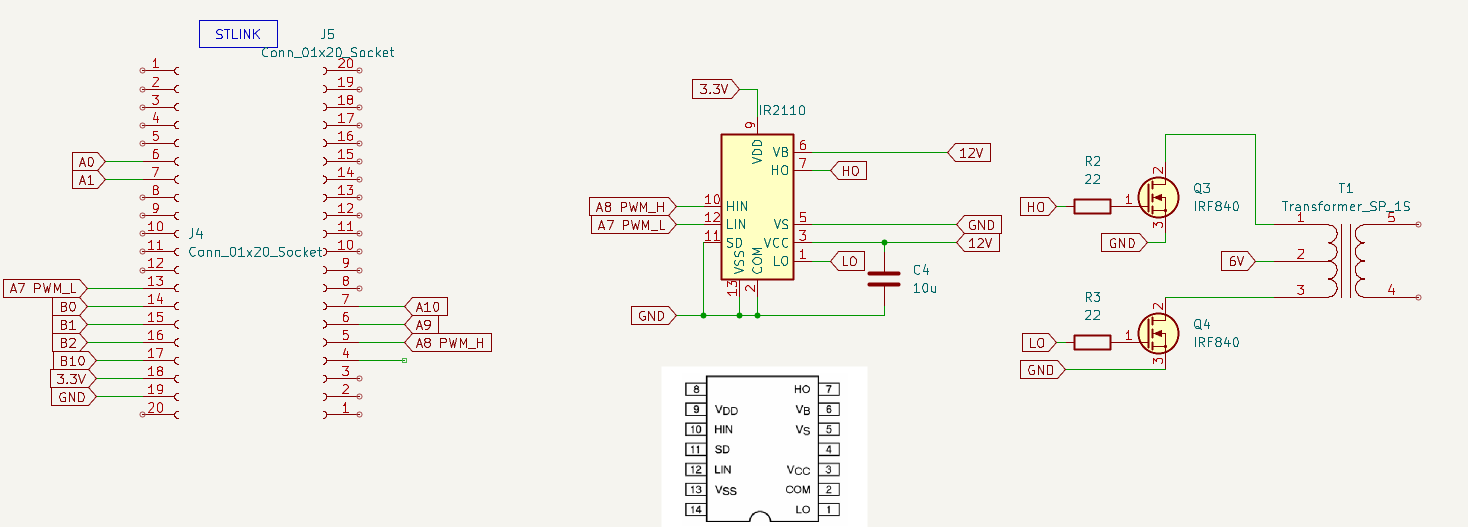
\includegraphics[width=\linewidth]{src/3Schematic.png}
\caption{Esquemático del circuito inversor implementado.}
\label{fig:esq}
\end{figure}

\begin{figure}[!h]
\centering
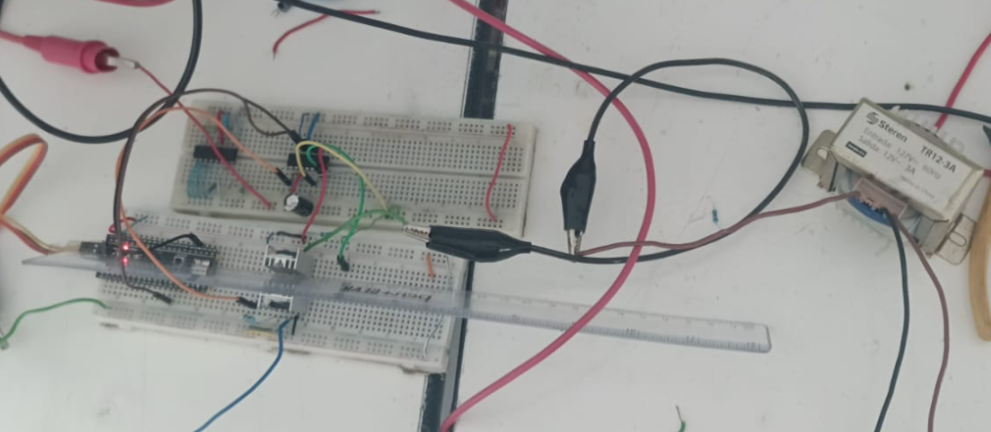
\includegraphics[width=0.8\linewidth]{src/EX3CIrcuit.png}
\caption{Circuito implementado con la etapa de control y potencia.}
\label{fig:cir}
\end{figure}

\subsection{Validación mediante Simulación}

Previo a la integración del prototipo físico, se efectuó un análisis de simulación en el software LTSpice con el propósito de validar la lógica de control y el acoplamiento magnético del sistema. El modelo incorporó los parámetros dinámicos de los MOSFET IRF840 y un transformador acoplado con inductancia mutua simétrica. Las formas de onda obtenidas en los nodos de salida confirmaron un nivel de tensión eficaz dentro del umbral esperado cercano a los $127{.}0\,\mathrm{V}$, corroborando la validez del diseño teórico propuesto.

\begin{figure}[!h]
\centering
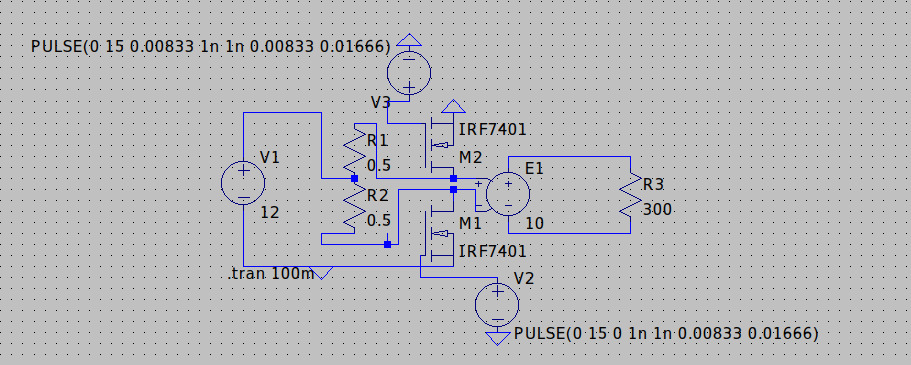
\includegraphics[width=0.8\linewidth]{src/spice.png}
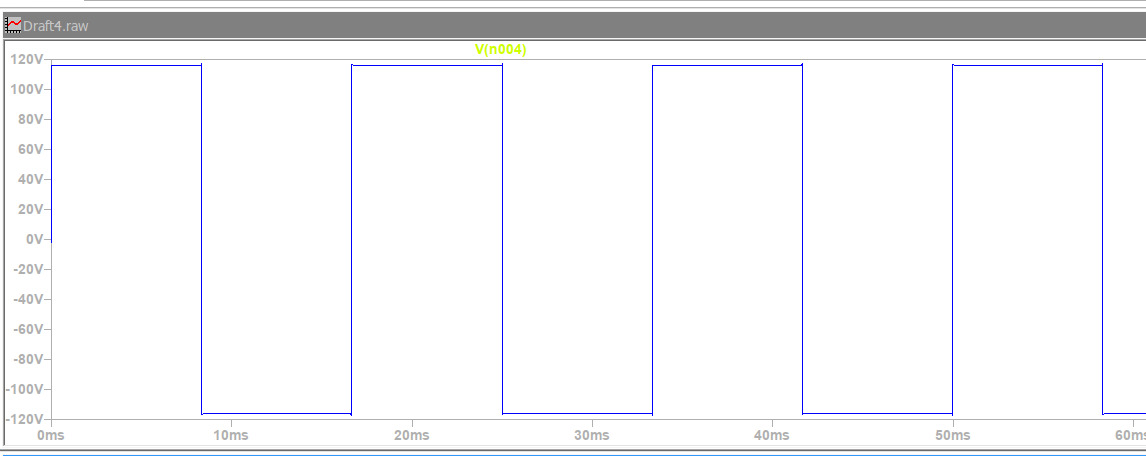
\includegraphics[width=0.8\linewidth]{src/simul.png}
\caption{Simulación LTSpice.}
\label{fig:placeholder}
\end{figure}

\subsection{Validación Experimental}

Una vez ensamblado el módulo de potencia, se realizaron las pruebas experimentales alimentando el sistema con una fuente regulada a $12{.}0\,\mathrm{V}$ en corriente directa y conectando un foco incandescente de $10{.}0\,\mathrm{W}$ como carga en el devanado secundario. El comportamiento de la señal de salida se monitoreó por medio de un osciloscopio digital utilizando sondas de prueba con atenuación de factor $10\times$. Los resultados gráficos de voltaje obtenidos en la carga se presentan en la Figura~\ref{fig:out}, donde se verifica la correcta entrega de potencia y la estabilidad en la frecuencia de operación.

\begin{figure}[!h]
\centering
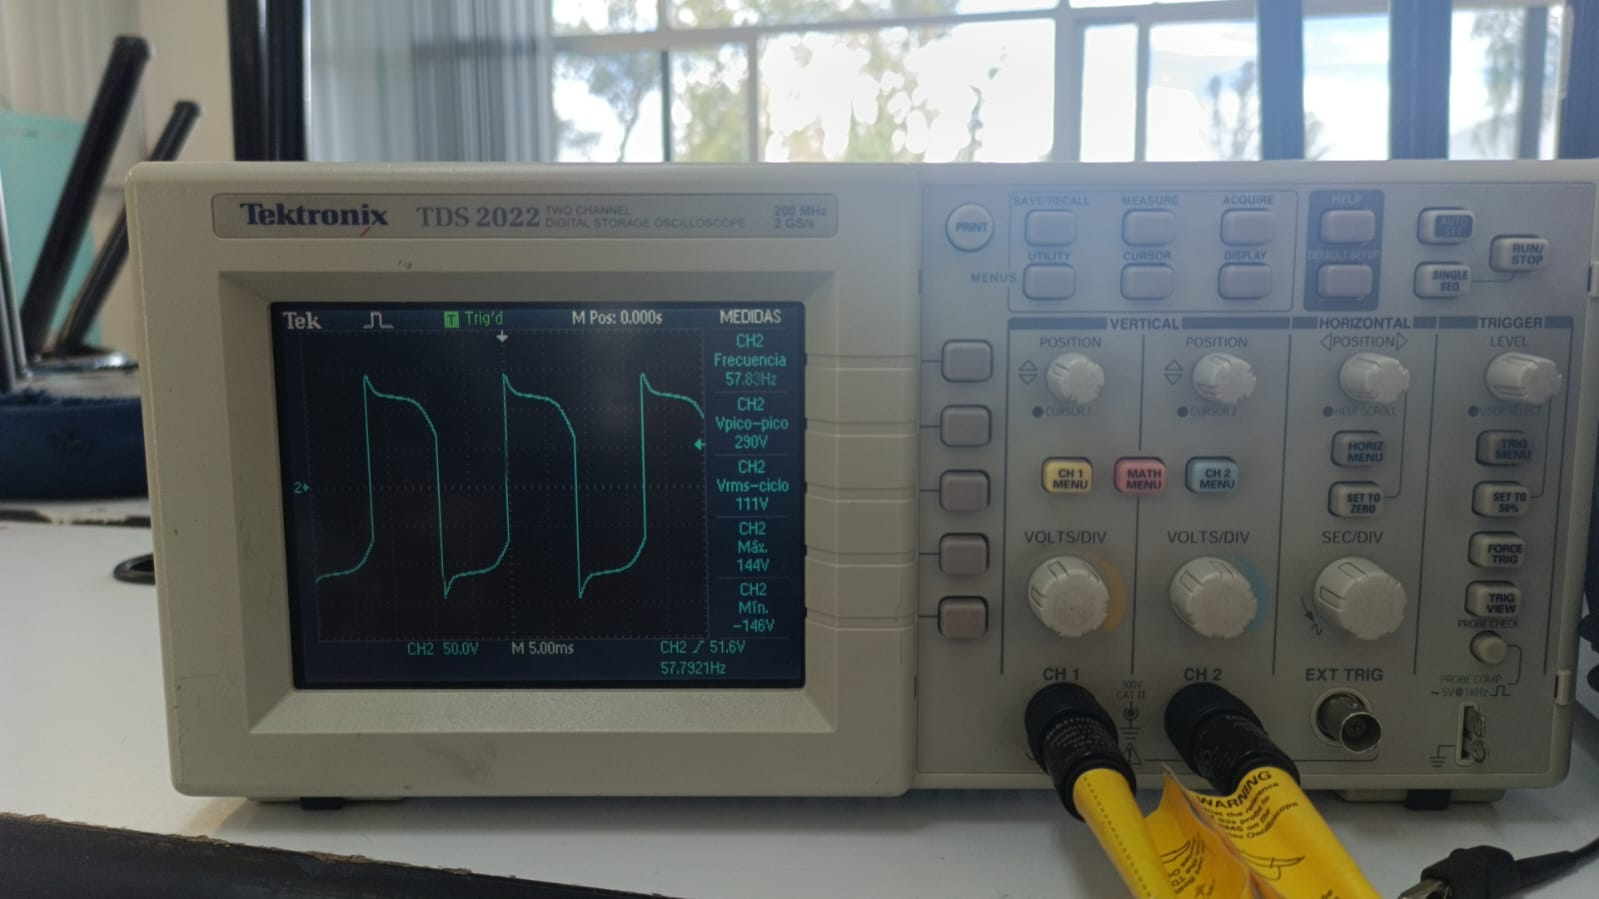
\includegraphics[width=0.7\linewidth]{src/EX3Salida.png}
\caption{Voltaje de corriente alterna obtenido en la carga durante las pruebas experimentales.}
\label{fig:out}
\end{figure}

\section{Discusión}

El desarrollo del proyecto permitió analizar de forma práctica los desafíos asociados a la conversión de energía eléctrica mediante conmutación push--pull. Las principales complicaciones durante la etapa de simulación se asociaron al ajuste de los tiempos muertos y a la correcta asignación de las referencias de tierra del driver de compuerta IR2110 en LTSpice, ya que las conexiones inadecuadas daban lugar a errores de convergencia matemática o a disparos erráticos en los transistores.\\

La experimentación evidenció las desviaciones naturales existentes entre los modelos ideales y la implementación física. A diferencia de las simulaciones, el circuito práctico presenta pérdidas por conducción dadas por la resistencia en estado activo $R_{\mathrm{DS(on)}}$ de los MOSFET, caídas de tensión en las conexiones y pérdidas magnéticas en el núcleo de hierro del transformador de $12{.}0\,\mathrm{V}$ a $3{.}0\,\mathrm{A}$. Estos fenómenos se traducen en una ligera disminución en el valor eficaz de la tensión final respecto a las estimaciones teóricas calculadas. El proceso de refinamiento en laboratorio facilitó la calibración de los registros del temporizador del microcontrolador STM32F411CEU para estabilizar el periodo fundamental en $16{.}66\,\mathrm{ms}$.\\

El prototipo construido constituye una base sólida para el estudio de sistemas de inversores monofásicos dentro de la Universidad Autónoma de Aguascalientes. Se logró cumplir el objetivo de elevar el voltaje para energizar una carga residencial típica de baja potencia. Como propuesta de mejora para trabajos futuros, se recomienda la incorporación de un filtro pasivo pasabajas tipo LC sintonizado a la frecuencia fundamental en el devanado secundario del transformador, lo que permitirá atenuar las componentes armónicas de alta frecuencia y aproximar la señal de salida a una onda senoidal pura.

\begin{thebibliography}{99}

\bibitem{ref1}
Hart, D. W. (2011). \textit{Inversores}. En Electrónica de potencia (pp. 331--386). McGraw-Hill.

\bibitem{ref2}
Rashid, M. H. (2015). \textit{Inversores monofásicos}. En Electrónica de potencia: circuitos, dispositivos y aplicaciones (4.a ed., pp. 245--292). Pearson Education.

\bibitem{ref3}
International Rectifier. (2005). \textit{Data Sheet No. PD60147: High and Low Side Driver IR2110(S)}.

\bibitem{ref4}
STMicroelectronics. (2020). \textit{RM0383 Reference Manual: STM32F411xC/E advanced ARM-based 32-bit MCUs}.

\bibitem{ref5}
Mohan, N., Undeland, T. M., \& Robbins, W. P. (2003). \textit{Switching dc-to-ac inverters}. En Power electronics: converters, applications, and design (3.a ed., pp. 200--248). John Wiley \& Sons.

\end{thebibliography}

\end{document}